\section{ISISDLM::File\-Repository Class Reference}
\label{classISISDLM_1_1FileRepository}\index{ISISDLM::FileRepository@{ISISDLM::FileRepository}}
{\tt \#include $<$File\-Repository.h$>$}

Collaboration diagram for ISISDLM::File\-Repository:\begin{figure}[H]
\begin{center}
\leavevmode

\includegraphics[width=120pt]{classISISDLM_1_1FileRepository__coll__graph}
\end{center}
\end{figure}
\subsection*{Public Member Functions}
\begin{CompactItemize}
\item 
int {\bf size} () const
\item 
{\bf i\-File::Iid} {\bf add\-Cube} (const std::string \&filename, Isis::Cube $\ast$cube, bool readonly=true)
\item 
{\bf i\-File::Iid} {\bf add\-Pvl} (const std::string \&filename, Isis::Pvl $\ast$pvl, bool readonly=true)
\item 
{\bf i\-File} $\ast$ {\bf get\-File} ({\bf i\-File::Iid} id)
\item 
{\bf i\-File} $\ast$ {\bf get\-Nth\-File} (int nth=0)
\item 
bool {\bf remove\-File} ({\bf i\-File::Iid} id)
\item 
void {\bf Purge} ()
\end{CompactItemize}
\subsection*{Static Public Member Functions}
\begin{CompactItemize}
\item 
{\bf File\-Repository} $\ast$ {\bf Instance} ()
\end{CompactItemize}
\subsection*{Static Public Attributes}
\begin{CompactItemize}
\item 
const char $\ast$const {\bf ID} = \char`\"{}\$Revision: 1.3 \$ \$Date: 2004/11/02 15:38:53 \$\char`\"{}
\begin{CompactList}\small\item\em Class version. \item\end{CompactList}\end{CompactItemize}
\subsection*{Protected Member Functions}
\begin{CompactItemize}
\item 
{\bf File\-Repository} ()
\end{CompactItemize}
\subsection*{Private Member Functions}
\begin{CompactItemize}
\item 
{\bf $\sim$File\-Repository} ()
\item 
{\bf File\-Repository} (const {\bf File\-Repository} \&k)
\item 
{\bf File\-Repository} {\bf operator=} (const {\bf File\-Repository} \&k)
\end{CompactItemize}
\subsection*{Private Attributes}
\begin{CompactItemize}
\item 
std::list$<$ {\bf i\-File} $\ast$ $>$ {\bf \_\-files}
\begin{CompactList}\small\item\em List of maintained files. \item\end{CompactList}\end{CompactItemize}
\subsection*{Static Private Attributes}
\begin{CompactItemize}
\item 
{\bf File\-Repository} $\ast$ {\bf \_\-instance} = 0
\begin{CompactList}\small\item\em Initialize the internal instance of itself. \item\end{CompactList}\end{CompactItemize}


\subsection{Detailed Description}
ISIS DLM File repository This class follows the classic Singleton pattern by the Gang Of Four (GOF). A discussion of this technique can be studied in their book {\em Design Patterns: Elements of Reusable Object-Oriented Software\/}.

This particular class serves as a holding tank for ISIS cube files and PVL like files. Although ISIS files have a PVL label, I distinguish between the two because they require different management schemes.

Isis labels are managed in real time in that all label manipulation is immediate. Any change that results in a modification of the the label content is immediately reflected in the file label (?).

PVL labels are contained within this repository until they are explicitly closed by the user or the program terminates and a purging of the repository is performed. 



\subsection{Constructor \& Destructor Documentation}
\index{ISISDLM::FileRepository@{ISISDLM::File\-Repository}!FileRepository@{FileRepository}}
\index{FileRepository@{FileRepository}!ISISDLM::FileRepository@{ISISDLM::File\-Repository}}
\subsubsection{\setlength{\rightskip}{0pt plus 5cm}ISISDLM::File\-Repository::File\-Repository ()\hspace{0.3cm}{\tt  [inline, protected]}}\label{classISISDLM_1_1FileRepository_b0}


\index{ISISDLM::FileRepository@{ISISDLM::File\-Repository}!~FileRepository@{$\sim$FileRepository}}
\index{~FileRepository@{$\sim$FileRepository}!ISISDLM::FileRepository@{ISISDLM::File\-Repository}}
\subsubsection{\setlength{\rightskip}{0pt plus 5cm}ISISDLM::File\-Repository::$\sim${\bf File\-Repository} ()\hspace{0.3cm}{\tt  [private]}}\label{classISISDLM_1_1FileRepository_d0}




Here is the call graph for this function:\begin{figure}[H]
\begin{center}
\leavevmode
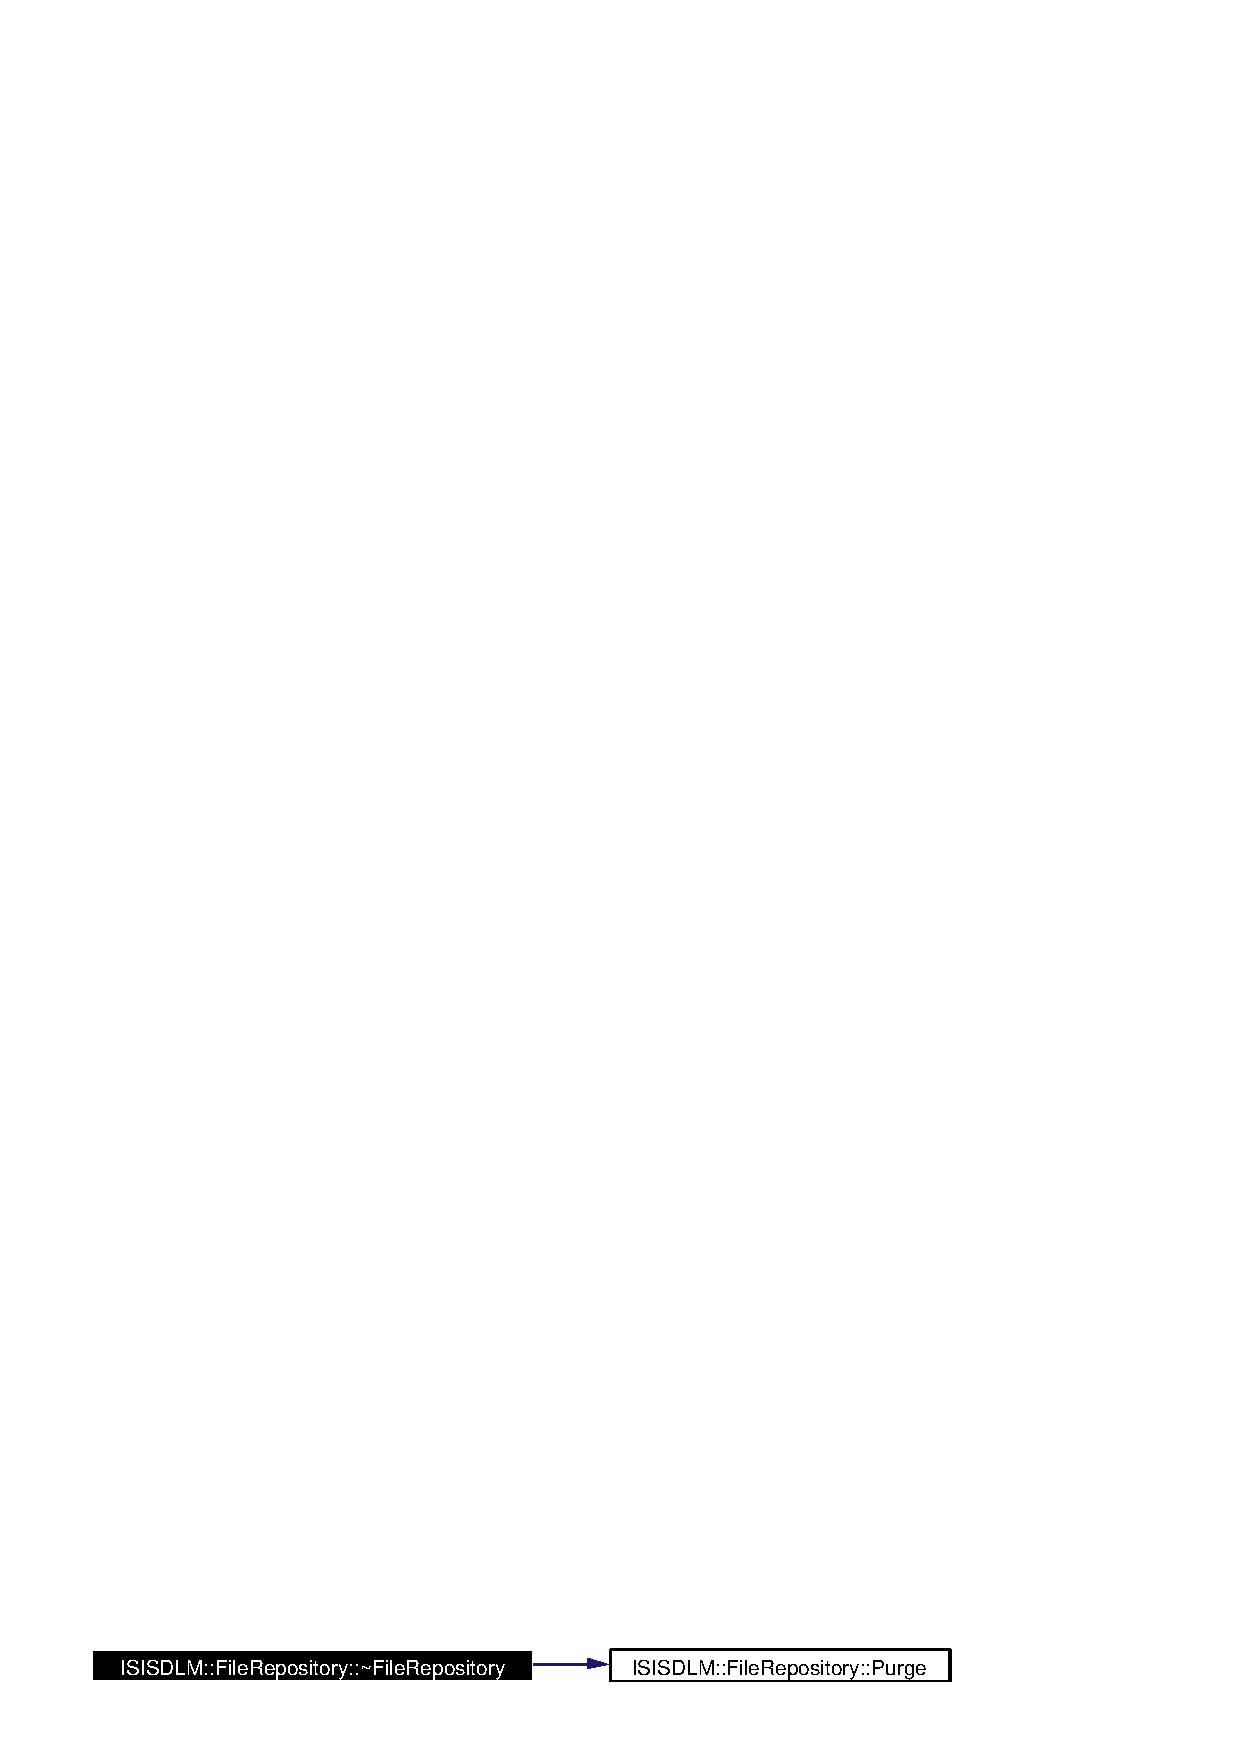
\includegraphics[width=232pt]{classISISDLM_1_1FileRepository_d0_cgraph}
\end{center}
\end{figure}
\index{ISISDLM::FileRepository@{ISISDLM::File\-Repository}!FileRepository@{FileRepository}}
\index{FileRepository@{FileRepository}!ISISDLM::FileRepository@{ISISDLM::File\-Repository}}
\subsubsection{\setlength{\rightskip}{0pt plus 5cm}ISISDLM::File\-Repository::File\-Repository (const {\bf File\-Repository} \& {\em k})\hspace{0.3cm}{\tt  [private]}}\label{classISISDLM_1_1FileRepository_d1}




\subsection{Member Function Documentation}
\index{ISISDLM::FileRepository@{ISISDLM::File\-Repository}!addCube@{addCube}}
\index{addCube@{addCube}!ISISDLM::FileRepository@{ISISDLM::File\-Repository}}
\subsubsection{\setlength{\rightskip}{0pt plus 5cm}{\bf i\-File::Iid} ISISDLM::File\-Repository::add\-Cube (const std::string \& {\em filename}, Isis::Cube $\ast$ {\em cube}, bool {\em readonly} = true)}\label{classISISDLM_1_1FileRepository_a1}




Here is the call graph for this function:\begin{figure}[H]
\begin{center}
\leavevmode

\includegraphics[width=187pt]{classISISDLM_1_1FileRepository_a1_cgraph}
\end{center}
\end{figure}
\index{ISISDLM::FileRepository@{ISISDLM::File\-Repository}!addPvl@{addPvl}}
\index{addPvl@{addPvl}!ISISDLM::FileRepository@{ISISDLM::File\-Repository}}
\subsubsection{\setlength{\rightskip}{0pt plus 5cm}{\bf i\-File::Iid} ISISDLM::File\-Repository::add\-Pvl (const std::string \& {\em filename}, Isis::Pvl $\ast$ {\em pvl}, bool {\em readonly} = true)}\label{classISISDLM_1_1FileRepository_a2}




Here is the call graph for this function:\begin{figure}[H]
\begin{center}
\leavevmode
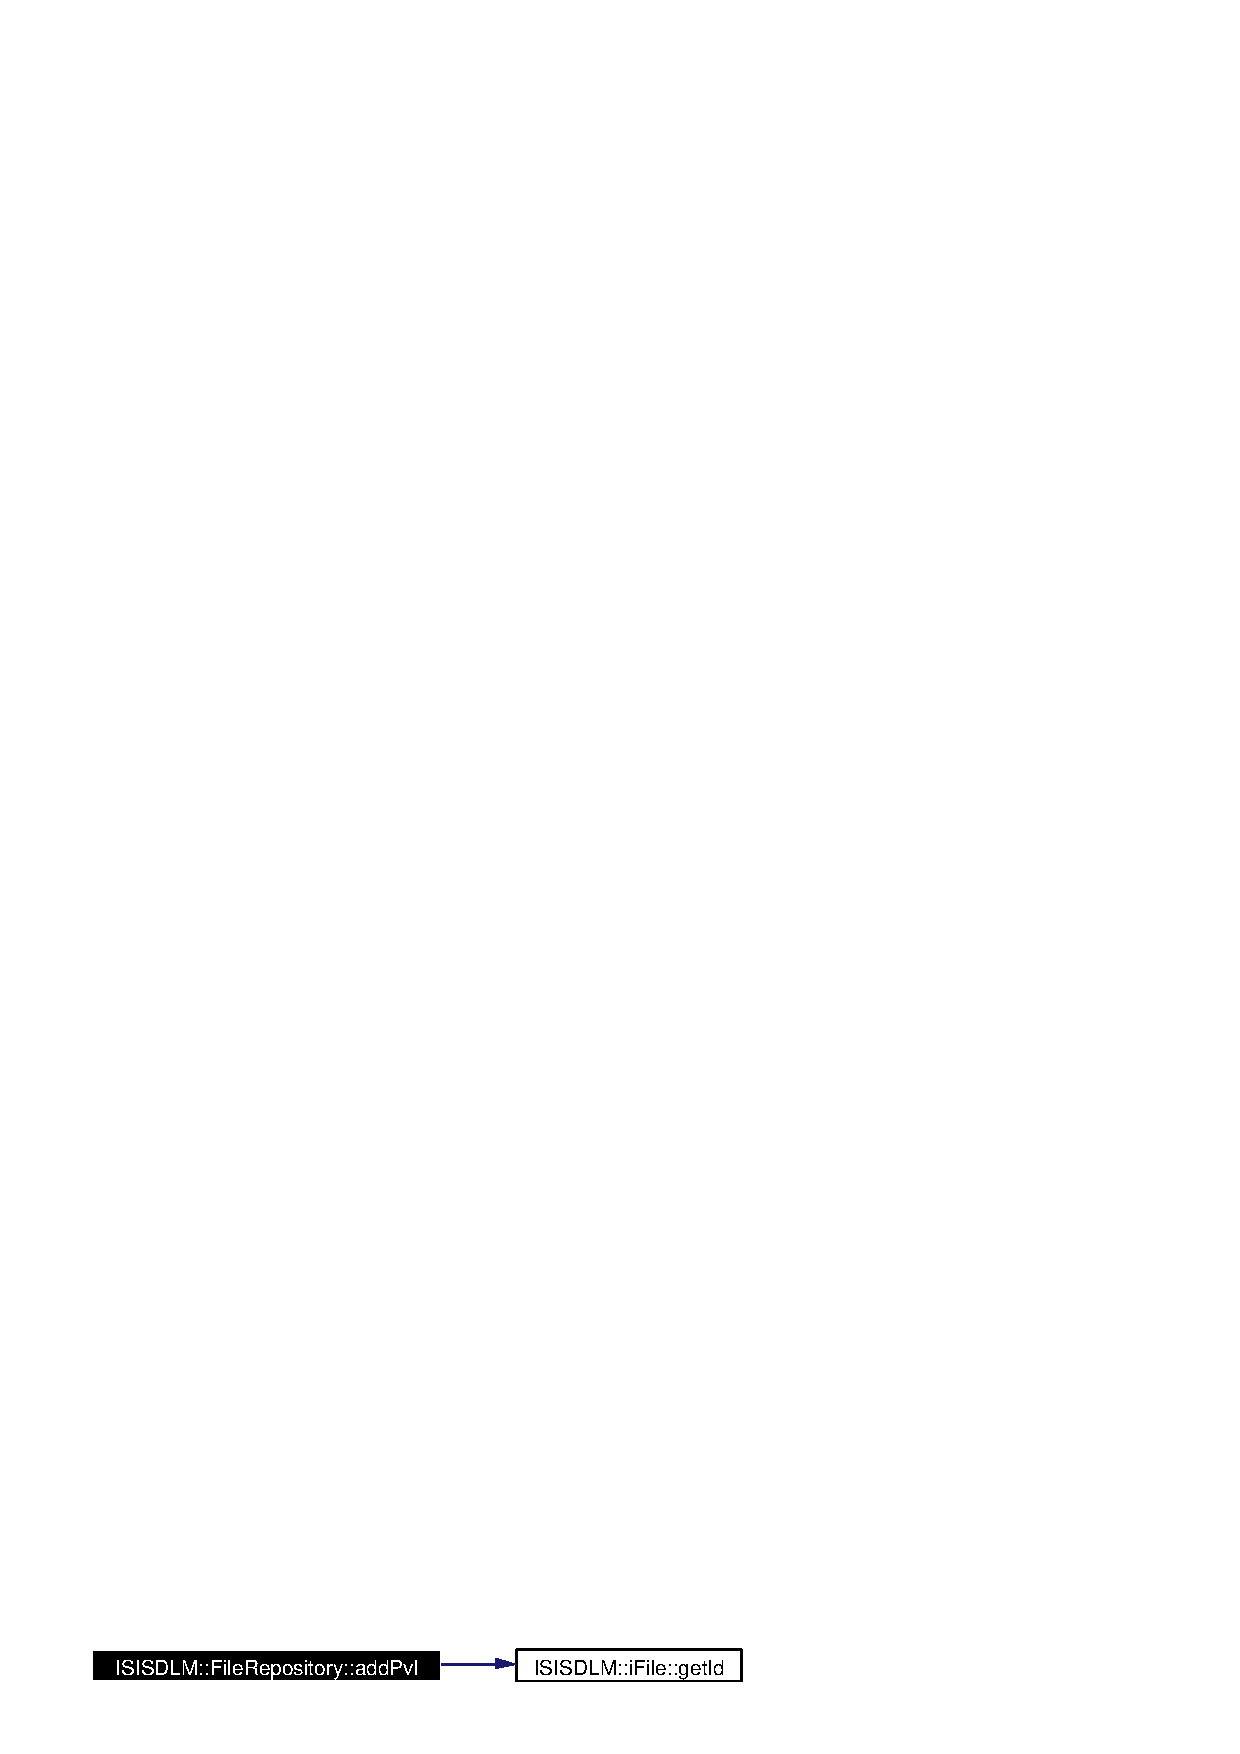
\includegraphics[width=182pt]{classISISDLM_1_1FileRepository_a2_cgraph}
\end{center}
\end{figure}
\index{ISISDLM::FileRepository@{ISISDLM::File\-Repository}!getFile@{getFile}}
\index{getFile@{getFile}!ISISDLM::FileRepository@{ISISDLM::File\-Repository}}
\subsubsection{\setlength{\rightskip}{0pt plus 5cm}{\bf i\-File} $\ast$ ISISDLM::File\-Repository::get\-File ({\bf i\-File::Iid} {\em id})}\label{classISISDLM_1_1FileRepository_a3}


\index{ISISDLM::FileRepository@{ISISDLM::File\-Repository}!getNthFile@{getNthFile}}
\index{getNthFile@{getNthFile}!ISISDLM::FileRepository@{ISISDLM::File\-Repository}}
\subsubsection{\setlength{\rightskip}{0pt plus 5cm}{\bf i\-File} $\ast$ ISISDLM::File\-Repository::get\-Nth\-File (int {\em nth} = 0)}\label{classISISDLM_1_1FileRepository_a4}


\index{ISISDLM::FileRepository@{ISISDLM::File\-Repository}!Instance@{Instance}}
\index{Instance@{Instance}!ISISDLM::FileRepository@{ISISDLM::File\-Repository}}
\subsubsection{\setlength{\rightskip}{0pt plus 5cm}{\bf File\-Repository} $\ast$ ISISDLM::File\-Repository::Instance ()\hspace{0.3cm}{\tt  [static]}}\label{classISISDLM_1_1FileRepository_e0}


The unique access method This method is the one and only one method that provides access to this object. It maintains an instance of itself by checking to see if the \_\-instance variable is defined. If not it creates an instance of itself and returns a pointer.

Note that the destructor is private to disallow user to delete it. This is forcibly maintained by the compiler. \index{ISISDLM::FileRepository@{ISISDLM::File\-Repository}!operator=@{operator=}}
\index{operator=@{operator=}!ISISDLM::FileRepository@{ISISDLM::File\-Repository}}
\subsubsection{\setlength{\rightskip}{0pt plus 5cm}{\bf File\-Repository} ISISDLM::File\-Repository::operator= (const {\bf File\-Repository} \& {\em k})\hspace{0.3cm}{\tt  [private]}}\label{classISISDLM_1_1FileRepository_d2}


\index{ISISDLM::FileRepository@{ISISDLM::File\-Repository}!Purge@{Purge}}
\index{Purge@{Purge}!ISISDLM::FileRepository@{ISISDLM::File\-Repository}}
\subsubsection{\setlength{\rightskip}{0pt plus 5cm}void ISISDLM::File\-Repository::Purge ()}\label{classISISDLM_1_1FileRepository_a6}


\index{ISISDLM::FileRepository@{ISISDLM::File\-Repository}!removeFile@{removeFile}}
\index{removeFile@{removeFile}!ISISDLM::FileRepository@{ISISDLM::File\-Repository}}
\subsubsection{\setlength{\rightskip}{0pt plus 5cm}bool ISISDLM::File\-Repository::remove\-File ({\bf i\-File::Iid} {\em id})}\label{classISISDLM_1_1FileRepository_a5}


\index{ISISDLM::FileRepository@{ISISDLM::File\-Repository}!size@{size}}
\index{size@{size}!ISISDLM::FileRepository@{ISISDLM::File\-Repository}}
\subsubsection{\setlength{\rightskip}{0pt plus 5cm}int ISISDLM::File\-Repository::size () const\hspace{0.3cm}{\tt  [inline]}}\label{classISISDLM_1_1FileRepository_a0}




\subsection{Member Data Documentation}
\index{ISISDLM::FileRepository@{ISISDLM::File\-Repository}!_files@{\_\-files}}
\index{_files@{\_\-files}!ISISDLM::FileRepository@{ISISDLM::File\-Repository}}
\subsubsection{\setlength{\rightskip}{0pt plus 5cm}std::list$<${\bf i\-File} $\ast$$>$ {\bf ISISDLM::File\-Repository::\_\-files}\hspace{0.3cm}{\tt  [private]}}\label{classISISDLM_1_1FileRepository_r0}


List of maintained files. 

\index{ISISDLM::FileRepository@{ISISDLM::File\-Repository}!_instance@{\_\-instance}}
\index{_instance@{\_\-instance}!ISISDLM::FileRepository@{ISISDLM::File\-Repository}}
\subsubsection{\setlength{\rightskip}{0pt plus 5cm}{\bf File\-Repository} $\ast$ {\bf ISISDLM::File\-Repository::\_\-instance} = 0\hspace{0.3cm}{\tt  [static, private]}}\label{classISISDLM_1_1FileRepository_v0}


Initialize the internal instance of itself. 

\index{ISISDLM::FileRepository@{ISISDLM::File\-Repository}!ID@{ID}}
\index{ID@{ID}!ISISDLM::FileRepository@{ISISDLM::File\-Repository}}
\subsubsection{\setlength{\rightskip}{0pt plus 5cm}const char $\ast$const {\bf ISISDLM::File\-Repository::ID} = \char`\"{}\$Revision: 1.3 \$ \$Date: 2004/11/02 15:38:53 \$\char`\"{}\hspace{0.3cm}{\tt  [static]}}\label{classISISDLM_1_1FileRepository_s0}


Class version. 



The documentation for this class was generated from the following files:\begin{CompactItemize}
\item 
{\bf File\-Repository.h}\item 
{\bf File\-Repository.cpp}\end{CompactItemize}
